% Copyright (C) 2012 The ESPResSo project
%  
% This file is part of ESPResSo.
%   
% ESPResSo is free software: you can redistribute it and/or modify it
% under the terms of the GNU General Public License as published by the
% Free Software Foundation, either version 3 of the License, or (at your
% option) any later version.
%  
% ESPResSo is distributed in the hope that it will be useful, but
% WITHOUT ANY WARRANTY; without even the implied warranty of
% MERCHANTABILITY or FITNESS FOR A PARTICULAR PURPOSE.  See the GNU
% General Public License for more details.
%  
% You should have received a copy of the GNU General Public License
% along with this program.  If not, see <http://www.gnu.org/licenses/>.
%
\newcommand{\taumax}{\tau_{\mathrm{max}}}
\newcommand{\taumin}{\tau_{\mathrm{min}}}

\chapter{Analysis in the core}
\label{chap:analysis-core}
\index{Analysis in the Core}

\section{Correlations and observables}
\index{Correlations}
\index{Observables}

\subsection{Introduction to the concept}
There is a fundamental difference between the observables defined in this
section and in the previous one. All the observables computed using the
\lit{analyze} command were temporary variables in the simulation kernel
and ceased to exist when they were returned to the script level.
The new concept of observables defined by the \lit{observable} command
creates variables in the kernel which exist for the entire simulation 
and when desired, their value is updated and either returned at the 
script level, or used by the kernel for further processing.
The ultimate goal of the whole framework is to provide a tool for
data processing on the fly. This is often desirable for 
the calculation of correlation functions. 

In general, a correlation function is any function of the form
\begin{equation}
C(\tau) = \left<A\left(t\right) \otimes B\left(t+\tau\right)\right>\,,
\label{eq:CtauDef}
\end{equation}
where $t$ is time, $\tau$ is the time difference between the moments
when the observables $A$ and $B$ were measured and $\otimes$ is an
arbitrary operator which produces a vector quantity 
$C$ from the two vectors $A$ and $B$. The ensemble averaging $\left< \cdot \right>$
implies averaging over all time origins $t$ and when applicable also
over realizations of observables $A$ and $B$ within individual configurations.
When both $A$ and $B$ are
the same quantity, $C(\tau)$ is called the autocorrelation, 
in the opposite case it is called the cross-correlation.

A stanadard example of an autocorrelation function is the velocity
autocorrelation function (vacf) and other correlation functions
which are useful in the Green-Kubo relations. In this case the observables
are particle velocities and the opeartion is scalar product.
The mean-square displacement (msd) is formally the same category of
a function, but now the observables are particle positions and
the operation is the square distance. 

In general, correlation functions
contain information on dynamics of the system. A typical vacf of a 
simple liquid oscillates and its envelope decays to zero beyond the 
time scale of molecular collisions.
To obtain it, one has to sample the velocities at very short intervals,
typically every timestep. If this should be done through the script interface
of \es, a significant part of cpu time would be spent on passing the control
from script to kernel and back. In more complex systems, the physically relevant 
part of correlation functions may span many orders of magnitude, ranging
from the time step to the total simulation time. In such cases offline
analysis is not possible becasue there is not enough space on the hard
drive to store the data. In addition to that, the trivial correlation algorithm
scales as $(\tau_{\mathrm{min}}/\tau_{\mathrm{max}})^2$ and if $\tau$
should span several orders of magnitude, the computation of correlation
functions may easily consume more cpu time than the actual simulation.
\es now features an efficient multiple tau correlation algorithm which
allows for computation of correlation functions over many orders of magnitude.
It is described in more detail in section~\ref{sec:multipleTau}.

The generic correlation interface of \es may process either observables
defined in the kernel, or data which it reads from an external file
or values entered through the scripting interface. 
\todo{Processing data from TCL input or from input files is not
  fully supported yet.}
Thus, apart from
data processing on the fly, it can also be used as an efficient correlator
for data produced by other programs. In all cases it produces a matrix of 
$n+2$ columns. The first two columns are the values of $\tau$ and 
the number of samples takes for a particular value of $\tau$ and the
remaining ones are the elements of the $n$-dimensional $C(\tau)$.


An example of the usage of observables and correlations is provided 
in the script \lit{correlation.tcl} in the samples directory.

\subsection{Observables}
\label{ssec:observable}
\newescommand{observable}
\index{Observables}

The following lines describe a generic call to work with 
observables. Different observables may require different further parameters.
\begin{essyntax}
  \variant{1} observable new \var{name} \opt{\var{parameters+}}
  \variant{2} observable \var{id} print \opt{formatted}
  \variant{3} observable \var{id} delete
\end{essyntax}
  
\variant{1} 
Defines a new observable and returns an integer $id$ which has been assigned to it.
The keyword \var{name} and the parameters have to correspond to one of the
observables described below.

\variant{2} Prints the value of the observable with a given $id$. If the observable
refers to the current state of the system, its value is updated before printing.
\todo{Formatted printing is not fully supported yet.}

\variant{3} Deletes the observable and makes the $id$ free for a new one.
\todo{Does not work yet}

\subsubsection{Implemented observables and their arguments}
Currently the following observables are implemented.
Particle specifications define a group of particles, from which
the observable should be calculated. They are generic to all 
observables and are described after the list of observables.

\todo{Missing descriptions of parameters of several observables}
  \begin{itemize}
    \item \lit{particle_positions} \var{particle\_specifications}\\
          Positions of the particles, in the format 
          $x_1,\ y_1,\ z_1,\ x_2,\ y_2,\ z_2,\ \dots\ x_n,\ y_n,\ z_n$. The particles 
          are ordered ascending according to their ids.
    \item \lit{particle_velocities} \var{particle\_specifications}\\
          Velocities of the particles, in the format\\ 
          $v^x_1,\ v^y_1,\ v^z_1,\ v^x_2,\ v^y_2,\ v^z_2,\ 
          \dots\ v^x_n,\ v^y_n,\ v^z_n$. 
          The particles are ordered ascending according to their ids.
    \item \lit{com_velocity} \var{particle\_specifications}\\
          Velocity of the centre of mass
    \item \lit{com_position} \var{particle\_specifications}\\
          Position of the centre of mass
    \item \lit{stress_tensor} \\
          The stress tensor. It only works with all particles. 
          It is returned as a 9-dimensional array:\\
          $ \{\ \sigma_{xx},\ \sigma_{xy},\ \sigma_{xz},\ \sigma_{yx},\ \sigma_{yy},\
          \sigma_{yz},\ \sigma_{zx},\ \sigma_{zy},\ \sigma_{zz}\ \} $
    \item \lit{stress_tensor_acf_obs} \\
          The observable for computation of the Stress tensor autocorrelation function. 
          Same as stress tensor, it only works with all particles.
          It is returned as a 6-dimensional array:\\
          $ \{\ \sigma_{xy},\ \sigma_{yz},\ \sigma_{zx},\ 
          ( \sigma_{xx} - \sigma_{yy}),\ 
          ( \sigma_{xx} - \sigma_{zz}),\ 
          ( \sigma_{yy} - \sigma_{zz})\  
          \} $ \\
          where $\sigma_{ij}$ are the components of the stress tensor.
    \item \lit{particle_currents} \var{particle\_specifications}\\
    \item \lit{currents} \var{particle\_specifications}\\
    \item \lit{dipole_moment} \var{particle\_specifications}\\
    \item \lit{structure_factor} \var{particle\_specifications}\\
    \item \lit{interacts_with} \var{particle\_specifications\_1} \var{particle\_specifications\_2} \var{cutoff} \\
          For each particle belonging to \var{particle\_specifications\_1} 
          the observable is unity if a neighbour of a type from 
          \var{particle\_specifications\_2} is found within the distance 
          defined by the \var{cutoff}. If no such neighbour is found, the 
          observable is zero. The observable has as one dimension per each 
          particle of \var{particle\_specifications\_1}
    \item \lit{nearest_neighbour_conditional} \\
          For each particle belonging to \var{type\_list\_1} return the particle id
	  of the nearest neighbour which has a particle type from \var{type\_list\_2}. 
	  If no such neighbour is found within the \var{cutoff}, it returns -1. 
	  The observable has 2 dimensions per particle of \var{type\_list\_1}. First
	  value is the neighbour id, the second one is the condition. Condition is
	  incremented when the particle state changes from \emph{no partners}
	  to \emph{some partner} or vice versa. In addition, in the former case
	  also the sign is changed.
          
    \item \lit{density_profile}
    \item \lit{lb_velocity_profile}
    \item \lit{radial_density_profile}
    \item \lit{radial_flux_density_profile}
    \item \lit{flux_density_profile}
    \item \lit{lb_radial_velocity_profile}
    \item \lit{textfile \var{textfilename} \opt{\var{column\_1} \dots \var{column\_n} }}
      This option allows to read data from an arbitrary text file, organized in columns.
      The name of the textfile is 
      \todo{Texfile input observable not fully supported yet!}
    \item \lit{tclinput \var{dimQ} } TCL input of length  \var{dimQ} is used as ``observable''. 
      \todo{Tcl input observable not fully supported yet!}
  \end{itemize}

\minisec{Particle specifications}
You can specify from which particles the observable should be computed in one of 
the following ways. In all cases, particle specifications refer to the current
state of espresso. Any later changes to particles (additions, deletions, changes
of types) will not be automatically reflected in the observable.
  \begin{itemize}
    \item \lit{all} \\
          Requests observable calculation based on all particles in the system.
    \item \lit{types} \var{ type\_list } \\
          Restricts observable calculation to a given particle type(s). The type
	  list is a tcl list of existing particle types.
    \item \lit{id} \var{ id\_list } \\
          Restricts observable calculation to a given list of particle id(s). The id 
	  list is a tcl list of existing particle ids.
% The following two particle specifications have not been implemented yet
%    \item \lit{blocks} \var{ m } \\
%          From an $n$-dimensional observable craeates an $n/m$-dimensional one by 
%	  averaging over $m$ neighbouring entries in the data array.
%      \todo{Not fully supported yet!}
%    \item \lit{strides} \var{ m } \\
%          From an $n$-dimensional observable craeates an $n/m$-dimensional one by 
%	  averaging over entries which are separated by $m$ in the data array.
%      \todo{Not fully supported yet!}
  \end{itemize}


\subsection{Correlations}
\label{ssec:correlations}
\newescommand{correlation}
\index{Correlations}

The observables defined by the \lit{observable} command can be used further 
to compute correlation functions. This requires some history of the observable values
to be stored in buffers and may consume a considerable amount of computer time.
The correlation first has to be defined by saying which observables 
are to be correlated, what should be the correlation operation, sampling
frequency, etc. When a correlation is defined, its id is returned which is
used further to do other operations with the correlation.
The general form is the following.
\begin{essyntax}
  \variant{0} correlation 
  \variant{1} correlation n_corr
  \variant{2} correlation \var{id} \{ update | autoupdate \{ start | stop\}  \}
  \variant{3} correlation \var{id} finalize
  \variant{4} correlation \var{id} print \opt{ average1 | variance1 | correlation_time | avarage_errorbars | spherically_averaged_sf }
  \variant{5} correlation \var{id} write_to_file \var{filname}
  \variant{6} correlation new obs1 \var{id1} \opt{obs2 \var{id2}} corr_operation \var{operation} dt \var{delta\_t} tau_max \var{tau\_max} \opt{tau_lin \var{tau\_lin}} \opt{compress1 \var{name} \opt{compress2 \var{name}} }
\end{essyntax}

Variants \variant{1} to \variant{5} operate only on existing
correlations. Variant\variant{6} creates an new correlation.
  
Variant \variant{0} returns a tcl list of the defined correlations
including their parameters.  \todo{Maybe not all parameters are
  printed.}  Variant \variant{1} returns the number of currently
defined correlations.  Variant \variant{2} starts or stops
automatically updating the correlation estimates (when using
\lit{autoupdate \{start | stop\}}. The update frequency is
automatically adjusted based based on the value of \var{dt} provided
when defining the correlation.  With \lit{update} it updates the
correlation estimates based on the instantaneous state of the system.
A correlation can be either in autoupdate or manual update regime but
not in both.  In the manual update mode it is the user's
responsibility to provide samples in the proper time interval. The
correlator has no way to check for it.  It is technically possible to
stop autoupdating and start updating manually but if you opt for it,
make sure that you exactly know what you are doing.

Variant \variant{3} correlates all data from history which are left in
the buffers. Once this has been done, the history is lost and no
further updates are possible. This operation improves the quality of
data in the tail of the  
correlation function if \var{tau\_max} is comparable to the total
simulation time. If \var{tau\_max} is much shorter, it does not
have much effect.

Variant \variant{4} returns the current status of the correlation
estimate as a Tcl variable. 

Variant \variant{5} writes the current status of the correlation
estimate to the specified filename. If the file exists, its contents will
be owerwritten.

Variant \variant{6} defines a new correlation and returns an integer
$id$ which has been assigned to it. Its further arguments are
described below.

\minisec{Output format} 

The output looks as follows:
\begin{code}
tau1 n_samples C1 C2 ... Cn
tau2 n_samples C1 C2 ... Cn
\end{code}
Where each line corresponds to a given value of \lit{tau}, \lit{n_samples} is the number
of samples which contributed to the correlation at this level and $C_i$ are the individual
components of the correlation.


\begin{arguments}
\item \lit{obs1} and \lit{obs2} \\ 
  are ids of the observables A and B that are to correlated. The ids have to refer to existing 
  observables which have been previously defined by the \lit{observable} command.
  Some observables are already implemented, and others can be easily added. This can be done
  with very limited \es{} knowledge just by following the implementations that are already
  in. If \lit{obs2} is omitted, autocorrelation of \lit{obs1} is calculated by default.
\item \lit{corr_operation} \\
  The operation that is performed on $A(t)$ and $B(t+\tau)$ to obtain $C(\tau)$. 
  The following operations are currently is available:
  \begin{itemize}
    \item \lit{scalar_product} \\
    Scalar product of $A$ and $B$, \ie $C=\sum\limits_{i} A_i B_i$
    \item \lit{componentwise_product} \\
    Comnponentwise product of $A$ and $B$, \ie $C_i = A_i B_i$
    \item \lit{square_distance_componentwise} \\
    Each component of the correlation vector is the square of the difference between the 
    corresponding components of the observables, \ie $C_i = (A_i-B_i)^2$. 
    Example: when $A$ is \lit{particle_positions}, it produces the mean square displacement
    (for each componnent separately).
    \item \lit{complex_conjugate_product}
    %\item List them here! \todo{write the list}
  \end{itemize}
\item \lit{dt} \\
  The time interval of sampling data points. When autoupdate is used, \var{dt} has
  to be a multiple of timestep. It is also used to produce time axis in real units.
  \textit{Warning: if \var{dt} is close to the timestep, autoupdate is strongly recommended.
  Otherwise cpu time is wasted on passing the control between the script and kernel.}
\item \lit{tau_max} \\
  This is the maximum value of $\tau$ for which the correlation should be computed.
  \textit{Warning: Unless you are using the multiple tau correlator, choosing \var{tau\_max}
  of more than 100\var{dt} will result in a huge computational overhead.
  In a multiple tau correlator with reasonable parameters, 
  \var{tau\_max} can span the entire simulation without
  too much additional cpu time.}
\item \lit{tau_lin} \\
  The number of datapoints for which the results are linearly spaced
  in tau.  This is a parameter of the multiple tau correlator. If you
  want to use it, make sure that you know how it works. By default, it
  is set equal to \var{tau\_max} which results in the trivial linear
  correlator. By setting \var{tau\_lin} < \var{tau\_max} the multiple
  tau correlator is switched on. In many cases, \var{tau\_lin}=16 is a
  good choice but this may strongly depend on the observables you are
  correlating.  For more information, we recommend to read
  Ref.~\cite{ramirez10a} or to perform your own tests.
\item \lit{compress1} and \lit{compress2} \\
  Are functions used to compress the data when going to the next level
  of the multiple tau correlator. Different compression functions for
  different observables can be specified if desired, otherwise the
  same function is used for both.  Default is \lit{discard} which
  takes one of the observable values and discards the other one. This
  is safe for all observables but produces poor statistics in the
  tail. For some observables, \lit{linear} compression can be used
  which makes an average of two neighbouring values but produces
  systematic errors.  Depending on the observable, the systematic
  error can be anything between harmless and disastrous. For more
  information, we recommend to read Ref.~\cite{ramirez10a} or to
  perform your own tests.
\end{arguments}

\subsubsection{Multiple tau correlator}
\label{sec:multipleTau}
\index{Multiple tau correlator}

Here we briefly describe the multiple tau correlator which is implemented in \es.
For a more detailed description and discussion of its behaviour with respect to
statistical and systematic errores, please read the cited literature.
This type of correlator has been in use for years in the analysis of
dynamic light scattering~\cite{schatzel88a}. About a decade later it found its way
to the Fluorescence Correlation Spectroscopy (FCS)~\cite{magatti01a}.
Despite its obvious advantages, has been used scarcely by the simulation community.
Even a detailed description in the book of Frenkel and Smit~\cite{frenkel02b}
for the special case of the velocity autocorrelation function did not really
help spreading the message.

\begin{figure}[ht]
\begin{center} 
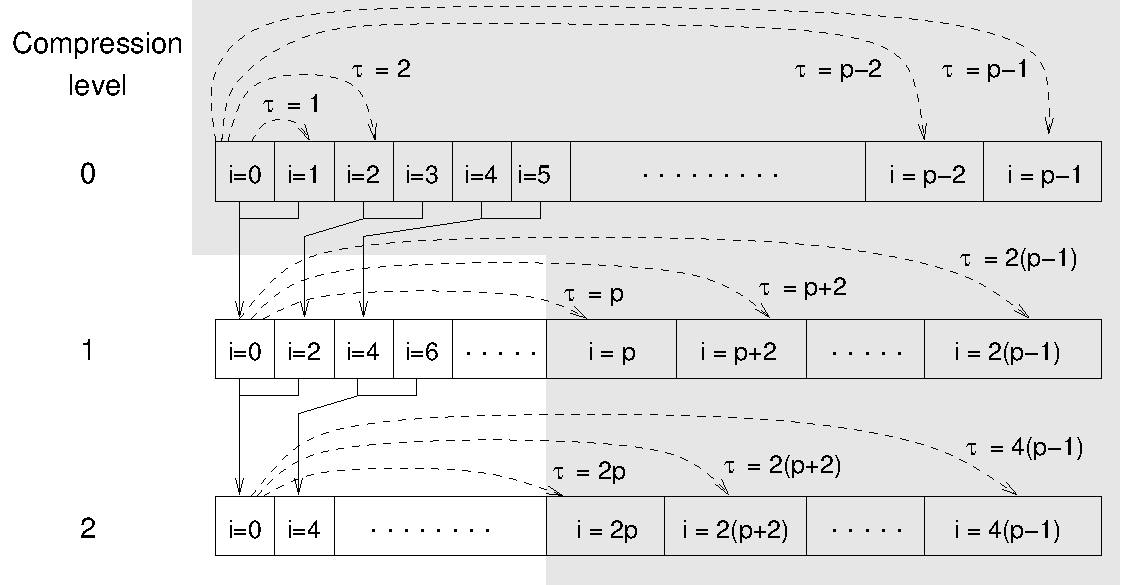
\includegraphics[width=0.9\textwidth]{figures/correlator_scheme}
\end{center} 
\caption{Schematic representation of buffers in the correlator.}
\label{fig:dataSet}
\end{figure}

Let us consider a set of $N$ observable values as schematically shown
in Figures~\ref{fig:dataSet}, where a value of index $i$ was measured
in time $i\delta t$. We are interested in computing the correlation 
function according to Equation~\ref{eq:CtauDef} for a range lag times
$\tau = (i-j)\delta t$ between the measurements $i$ and $j$.
To simplify the notation, we further drop $\delta t$
when refering to observables and lag times. 

The trivial implementation takes all possible pairs of values
corresponding to lag times $\tau \in [\taumin:\taumax]$. 
Without loss of generality, let us further consider $\taumin=0$.
The computational effort for such an algorithm scales
as ${\cal O} \bigl(\taumax^2\bigr)$.
As a rule of thumb, this is feasible if $\taumax < 10^3$.
The multiple tau correlator provides a solution to compute the
correlation functions for arbitrary range of the lag times by
coarse-graining the high $\tau$ values. It applies the naive algorithm
to a relatively small range of lag times $\tau \in [0:p-1]$. This we refer
to as compression level 0. To compute the correlations for lag times
$\tau \in [p:2(p-1)]$, the original data are first coarse-grained, so
that $m$ values of the original data are compressed to produce a single
data point in the higher compression level. Thus the lag time between
the neighbouring values in the higher compression level increases
by a factor of $m$, while the number of stored values decreases by
the same factor and the number of correlation operations at this level
reduces by a factor of $m^2$. Correlations for lag times 
$\tau \in [2p:4(p-1)]$ are computed at compression level 2, which is created
in an analogous manner from level 1. This can continue hierarchically
up to an arbitrary level for which enough data is available. Due to the
hierarchical reduction of the data, the algorithm scales as 
${\cal O} \bigl( p^2 \log(\taumax) \bigr)$. Thus an additional order
of magnitude in $\taumax$ costs just a constant extra effort.

The speedup is gained at the expense of statistical accuracy.
The loss of accuracy occurs at the compression step.
In principle one can use any value of $m$ and $p$ to tune the algorithm
performance. However, it turns out that using a high $m$ dilutes the
data at high $\tau$. Therefore $m=2$ is hardcoded in the \es correlator
and cannot be modified by user. The value of $p$ remains an adjustable
parameter which can be modified by user by setting \lit{tau_lin}
when defining a correlation. In genral, one should choose $p \gg m$
to avoid loss of statistical accuracy. Choosing $p=16$ seems to be
safe but it may depend on the properties of the analyzed
corerlation functions. A detailed analysis has been performed
in Ref.~\cite{ramirez10a}.

The choice of the compression function also influences the statistical
accuracy and can even lead to systematic errors. The default compression 
function is \lit{discard2} which discards the second fo the compressed 
values and pushes the first one to the higher level. This is robust and 
can be applied universally to any combination of observables and
correlation operation. On the other hand, it reduces the
statistical accuracy as the compression level increases.
In many cases, the \lit{average} compression operation
can be applied, which averages the two neighbouring values
and the average then enters the higher level, preserving
almost the full statistical accuracy of the original data. 
In general, if averaging can be safely used or not, depends on the 
properties of the difference
\begin{equation} 
\frac{1}{2} (A_i \otimes B_{i+p} + A_{i+1} \otimes B_{i+p+1} ) - 
\frac{1}{2} (A_i + A_{i+1} ) \otimes \frac{1}{2} (B_{i+p} +  B_{i+p+1})
\label{eq:difference}
\end{equation} 
For example in the case of velocity autocorrelation function, the
above-mentioned difference has a small value and a random sign, \ie\ 
different contributions cancel each other. On the other hand, in the
of the case of mean square displacmenent the difference is always positive,
resulting in a non-negligible systematic error. A more general
discussion is presented in Ref.~\cite{ramirez10a}.
